\documentclass{article}
\usepackage{geometry}
\usepackage{natbib}
\usepackage{amssymb}
\usepackage{amsmath}
\usepackage{graphicx}
\usepackage{hyperref}
\usepackage{textcomp}
\usepackage{array}
\usepackage{booktabs}
\usepackage{makecell}
\usepackage[singlelinecheck=false]{caption}

\geometry{
	a4paper,
	total={170mm,257mm},
	left=30mm,
	top=30mm,
	bottom=20mm,
	right=20mm
}
\title{
	Projeto de Iniciação Científica - Relatório 1\\
	Visualização Unidimensional do Espaço Tridimensional \\
	\large Prólogo para Visualização Bidimensional do Espaço Quadridimensional
}
\date{2023-06-28}
\author{Paulo Roberto Rodrigues da Silva Filho\\ \small Felipe Acker (Orientador)}

\newcommand\R{\mathbb{R}}

\begin{document}
	\renewcommand{\figurename}{Figura}
	\renewcommand{\tablename}{Tabela}
	\renewcommand{\cellalign}{tl}
	\renewcommand{\theadalign}{tl}
	
	\graphicspath{ {./imagens/} }
	\maketitle
	\tableofcontents
	
	\section{Introdução}
	
	\paragraph{}
	Atualmente, os algoritmos de Ray-Tracing, visualização e radiosidade, para projeção de espaços 3D em 2D estão dominados e tecnologicamente avançados, já tendo mesmo implementações em Hadware, através de placas de vídeo 3D \textit{\textbf{[adicionar referências]}}. Entretanto, tais técnicas implementam a representação do espaço tridimensional no espaço bidimensional, reduzindo apenas uma dimensão de representação, e apenas para o caso particular de $\R^3$. Entratanto, não há tecnologias consistentes que permitam a redução de $\R^3$ para $\R$, ou de $\R^4$ para $\R^2$ - objetivo final desse projeto.
	
	\paragraph{}
	Assim, foi necessário desenvolver a tecnologia e os algoritmos para essas representações da estaca zero. Esse relatório visa apresentar os cálculos necessários para prover tal renderização de objetos tridimensionais, em projeção unidimensional, utilizando o modelamento físico de olho, apresentado na proposta e na renderização de objetos quadridimensionais em projeção bidimensional.
	
	\paragraph{}
	O processo de irradiação luminosa e focalização é estendido do caso tridimensional para o caso quadridimensional, enquanto o processo de captura de imagem é reduzido do caso bidimensional para o caso unidimensional, nas projeções de $\R^3$ para $\R$, ou do caso tridimensional para o caso bidimensional, nas projeções de $\R^4$ para $\R^2$.
	
	\paragraph{}
	Em um primeiro momento, é entendido o processo de renderização de objetos bidimensionais em uma tela monodimensional, com a utilização de sombras, com o cálculo de radiosidade, mas sem a utilização completa de \textit{ray-tracing}, ou seja, não serão consideradas superfícies espelhadas. A partir daí, esse algoritmo é estendido para a renderização de objetos tridimensionais em tela monodimensional - que é o objetivo planejado para esse projeto - e, por último, esse algoritmo é estendido para a renderização de objetos quadridimensionais em telas bidimensionals, o que já seria o objetivo final do projeto. 
	
	\section{Modelo Mínimo - Ambiente Bidimensional em Tela Monodimensional} \label{modelo-minimo}
	
	\paragraph{}
	O modelo mínimo é a renderização de objetos bidimensionais em uma tela unidimensional. Esse modelo de renderização é \textbf{inferior} ao que já é implementado atualmente em software e em hardware, pelas placas 3D, mas é a base do modelo de renderização quadridimensional - portanto, entendê-lo é fundamental para a implementação de modelos de renderização que fujam do padronizado, que é a Renderização de Ambientes Tridimensionais em Telas Bidimensionais.
	
	\paragraph{}
	Para haver renderização, é necessário haver \textbf{iluminação} e \textbf{captura}. A captura é feita pelo olho, é já é uma característica da renderização assumida por definição. A iluminação, apesar de obrigatória para a renderização, não é imediatamente considerada pelo senso comum. Entretanto, renderização sem um modelo de iluminação adequada apresentaria figuras achatadas e sem volume aparente, que permitiria discernir sobre as formas representadas na renderização.
	
	\paragraph{}
	Usamos dois modelos de iluminação: \textbf{(1)} Iluminação Paralela, adequada para ambientes externos e \textbf{(2)} Iluminação radial, adequada para ambientes internos. Em ambos os casos adicionamos um componente de iluminação difusa. Não é apresentado o algoritmo de \textit{tinting}, então todas as fontes luminosas são brancas e não é apresentado o algoritmo para a utilização de mais de uma fonte luminosa. Essas omissões são corrigidas posteriormente, em uma seção específica para elas.	
	
	\subsection{Iluminação Paralela}
	
	\paragraph{}
	Na iluminação paralela de ambiente bidimensional, a fonte de luz é representada como uma reta que emite luz na direção perpendicular de sua linha - ou seja, nas suas normais, em todos os pontos. A estrutura de visualização possui seus elementos apresentandos nas Figuras \ref{fig:rend} e \ref{fig:radio}. A iluminação paralela assume que não há decaimento de intensidade, mas esse modelo não é necessariamente verdadeiro em todos os cenários. Para um melhor entendimento do modelamento da intensidade luminosa, a seção a seguir, \ref{intensidade-1}, apresenta o racional físico/geométrico da intensidade, e um modelo extendido de como lidar com a intensidade luminosa.
	
	\begin{figure}[h]
		\centering
		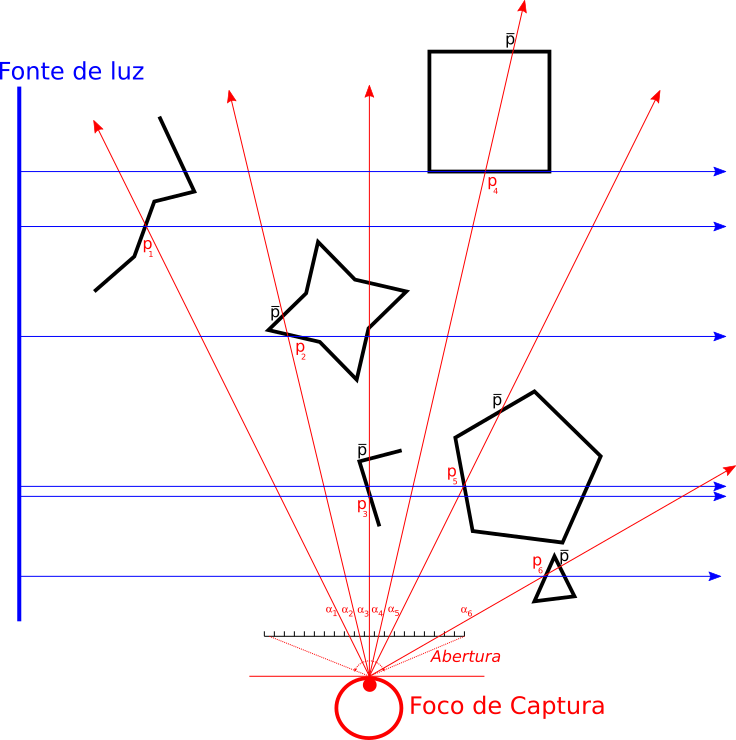
\includegraphics[scale=0.7]{Renderizacao-2D-1D}
		\caption{Identificando pontos de renderização. No inferior da figura temos o foco de captura, interceptado por uma tela unidimensional com vinte pixels de tamanho. À esquerda, temos uma fonte de luz paralela. Essa fonte de luz, na figura, está na vertical, mas qualquer direção do plano pode ser utilizada por tal fonte - desde que ela esteja longe o suficiente para nunca estar entre o foco de captura e os objetos visualizados.}
		\label{fig:rend}
	\end{figure}

	\subsubsection{Modelamento de Intensidade de Iluminação} \label{intensidade-1}
	
	\paragraph{}
	A intensidade luminosa é parte integrante do cálculo da radiosidade. No nosso mundo real (que é um mundo tridimensional), a intensidade luminosa representa a dispersão da \textbf{energia} dispersada por uma fonte de luz, no tempo (ou seja, é uma medida de potência), por uma superfície. A unidade de intensidade luminosa é a \textbf{Candela}. \textit{\textbf{[adicionar referências]}}. 
	
	\paragraph{}
	Uma das características fundamentais do decaimento luminoso, em função da distância, é que se assume que a luz se dispersa pelo ângulo sólido no qual ela se propaga a partir de sua fonte central. Assim, nem de uma fonte de luz paralela, nem de fonte de luz coerente (como no caso dos \textit{lasers}), haveria decaimento de intensidade, mas em focos de luz ordinários, o decaimento seria com o quadrado da distância, pois essa é a taxa de crescimento da área da superfície do ângulo sólido, na medida em que nos distanciamos do centro de emissão da luz.
	
	\paragraph{}
	Para a renderização de imagens, a intensidade máxima de iluminação representa que nenhuma das cores da linha, superfície ou variedade iluminada possui qualquer tipo de desconto de brilho, por conta da distância da fonte de luz. Em ambientes bidimensionais, a taxa de decaimento da intensidade é dada linearmente, pois o ângulo plano representa um comprimento unidimensional. Em ambientes tridimensionais, a taxa de decaimento cai com o quadrado da distância e em ambientes quadridimensionais, estaríamos falando de um ângulo representado por uma 3-variedade e a taxa de decaimento seria com o cubo da distância.
	
	\paragraph{}
	De forma geral, a intensidade luminosa utilizada para a renderização de imagens pode ser dada por:
	
	\begin{equation} \label{eq:1}
	 I(D) = \frac{k}{(1+D)^n}, n = 1,2,3, ... 
	\end{equation}

	Assumindo que à distância 1 (em uma unidade arbitrária), da fonte de luz, a intensidade luminosa é, por definição, igual a 1, e há o decaimento exponencial a partir daí. Se essa assunção não for feita, haveriam casos de intensidade luminosa infinita, o que não seria estritamente errado, para $D = 0$, mas muito inconveniente, para fins de representação.
	
	\paragraph{}	
	O valor $k$ é uma constante de intensidade arbitrária (sendo o valor padrão $k=2$, enquanto o valor de $n$, acima, pode ser modulado, dependendo da conveniência da implementação, enquanto $D$ é, necessariamente, a distância entre o ponto visualizado e a fonte de luz. Podemos ter universos bidimensionais que desejamos que o decaimento da intensidade luminosa não seja linear, podendo ser quadrática, para esse universo bidimensional representar um corte de um universo tridimensional maior, ou o decaimento da intensidade luminosa pode ser linear, em um universo tridimensional, no qual a intensidade deixa de ser um aspecto geométrico da luz, passando a seguir alguma lei alternativa que seja conveniente para a representação visual deste mundo. Assim, a dimensão de decaimento da intensidade luminosa fica escolhida arbitrariamente caso a caso, segundo a conveniência da implementação do mundo.
	
	\subsubsection{Abertura de Visualização e Varredura de Pontos} \label{varredura-1}
	
	A Figura \ref{fig:rend} mostra o exemplo da captura de seis pixels por uma tela unidimensional, em um ambiente bidimensional, com fonte de luz paralela (ou seja, luz ambiente). Esse é o modelo mínimo, renderizando um ambiente bidimensional em uma tela unidimensional. Tal exemplo é utilizado para exemplificar os seguintes conceitos:
	
	\begin{enumerate}
		\item Ângulo de abertura de visão - Aplicação do \textbf{Critério da Abertura}
		\item Fonte de Luz - Aplicação do \textbf{Critério da Direção}
		\item Radiosidade - Aplicação do \textbf{Critério da Distância e da Direção}, mas para a Fonte de Luz
		\item Pontos visíveis e não visíveis - Aplicação do \textbf{Critério da Distância}
	\end{enumerate}
	
	\paragraph{}
    Na Figura \ref{fig:rend} mostra-se, logo acima do foco de captura, a tela unidimensional, com vinte pixels. Cada pixel é renderizado de acordo com as interseções dos raios de visão (representados pelas setas vermelhas) com os objetos que tais raios atravessam. Cada raio renderiza apenas \textbf{o ponto mais próximo} ao foco de captura. Essa condição faz parte do \textbf{Critério da Distância}. Assim, para os raios de visão $\alpha_1, ..., \alpha_6$, são renderizados os pontos $p_1, ..., p_6$, na tela. Esses pontos são aqueles mais próximos do foco de captura, e o que estiver para além deles, não é renderizável - ou seja, é invisível para o Foco de Captura. Assim, todos os pontos representados por $\bar{p}$ são invisíveis ao foco de captura e, portanto, não são renderizados.
    
    \paragraph{}
    Nas figuras \ref{fig:rend} e \ref{fig:rend-rad}, o foco de captura está centralizado no décimo-primeiro pixel, da esquerda para a direita. Isso é apenas para propósito de apresentação. Rigorosamente, foco deve estar localizado exatamente no meio da tela, mas isso tornaria a representação no desenho mais difícil. De toda forma, a posição da tela perante o foco de captura é totalmente arbitrário e pode mudar implementação a implementação. Nas outras figuras, a representação de tela está mais alinhada com o esperado para uma implementação real.
    
    \paragraph{}
    A renderização do ponto na tela, em si, é apenas a ativação e desativação de uma determinada cor naquele ponto de tela, ou \textbf{pixel}. O pixel não tem dimensão, e ou ele é integralmente representado, ou não - ficando apenas um ponto preto em sua posição\footnote{Essa regra não é tão rigorosa assim. Existem técnicas de \textit{anti-aliasing} que podem flexibilizar um pouco essas condições - entretanto, \textit{anti-aliasing} está além do escopo desse relatório e desse projeto.}. Se o raio de visão identifica quais pontos da tela serão ativados ou não, qual cor será ativada depende da cor do objeto representado e da radiosidade do ponto desse objeto que está sendo representado em tela.
    
	\begin{figure}[h]
		\centering
		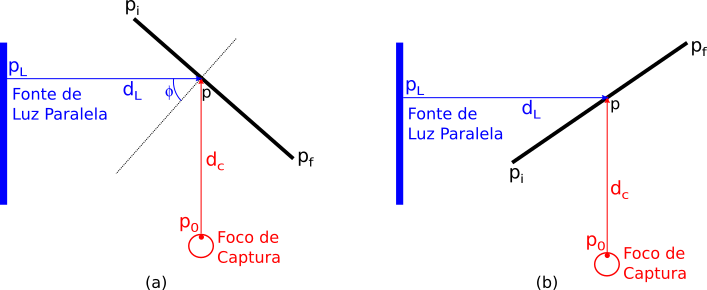
\includegraphics[scale=0.7]{radiosity}
		\caption{Identificando pontos de renderização.}
		\label{fig:radio}
	\end{figure}

	\paragraph{}
	O primeiro critério a ser considerado para haver iluminação de um ponto visível por estar diretamente exposto ao raio de visão é verificar se ele também está diretamente exposto a um raio de luz proveniente da fonte. No caso da fonte de luz paralela, considera-se uma reta paralela, mas normal à Fonte de Luz, que estará posicionada em um local infinitamente\footnote{Na verdade, esse foco de luz paralelo precisa estar em um ponto \textbf{convenientemente} distante, caso seja aplicado qualquer critério de decaimento de intensidade para os feixes paralelos de luz, em algum "universo" ficcional simulado, no qual as fontes paralelas de luz tenham tal comportamento.} distante, passando pelo ponto visualizado. Se esse ponto for o primeiro irradiado pelo raio de luz (ou se for a primeira interseção com algum objeto que seja atravessado por tal raio, considerando sua direção), então o ponto é iluminado. Observando a Figura \ref{fig:rend}, percebe-se que os pontos $p_1$, $p_2$, $p_3$ e $p_6$ são iluminados. Já o ponto $p_5$ não é iluminado porque seu raio de luz é interrompido pelo objeto que contém o ponto $p_3$, estando, portanto, em sombra. Já o ponto $p_4$ está em um segmento paralelo aos raios de luz, não recebendo iluminação, também. Outra justificativa de $p_4$ não ser iluminado é porque o primeiro ponto do segmento ao qual ele pertence é que é iluminado, e todos os outros pontos depois desse, considerando a direção do raio de luz, estão em sombra. 
	
	\paragraph{}
	Mas o ponto iluminado por ser o primeiro a ser irradiado precisa refletir o raio de luz recebido em direção ao foco de captura, para dizer que ele, o ponto visualizado, está sendo realmente iluminado. Assim, na Figura \ref{fig:radio} são mostradas as duas possibilidades de identificação de se um ponto visível por estar diretamente exposto ao raio de visão receberá iluminação ou não. Em \textit{\textbf{(a)}}, tanto o raio de visão, quanto o raio de iluminação estão diretamente acessando o ponto $p$, visualizado, e o ponto $p_l$ e $p_0$ estão do mesmo lado da reta $p_i$-$p_f$, que representa o objeto visualizado, que contém o ponto $p$. Nesse caso, o ponto $p$ é iluminado. Em \textit{\textbf{(b)}}, o ponto $p_l$ e o ponto $p_0$ estão em lados opostos da reta $p_i$-$p_f$. Já nesse caso, o ponto $p$ não é iluminado, porque ele reflete a luz recebida para uma direção fora do foco de captura. Assim, o ponto $p$ aparece em sombra.
	
	\subsubsection{Identificação, Iluminação e Coloração do Pixel - cálculos}
	
	\paragraph{}
	Uma vez identificado o ponto $p_i$ a ser renderizado e se ele está iluminado ou não, deve-se calcular a cor de tal ponto. Calculada a cor, ele pode ser renderizado na tela (unidimensional). Assume-se as informações iniciais da tabela \ref{tab:var}, em notação consistente com as figuras \ref{fig:rend}, \ref{fig:radio} , \ref{fig:rend-rad} e \ref{fig:radio-rad}. 
	
	\paragraph{Orientação Espacial:} Uma das informações mais relevantes para todos os cálculos apresentados aqui, em todas as dimensões apresentadas, é o fato de que os eixos de representação, com origem no ponto $p_0$, seguem a regra de que o primeiro eixo, $x$, parte de $p_0$ para o $+\infty$, na direção \textit{para frente}; e, \textit{para trás}, ele segue para o $-\infty$. O próximo eixo, $y$, ele segue para $+\infty$ na direção \textit{para a esquerda}, e os outros eixos ($z$ e $w$) são orientados de acordo com a \textbf{\textit{regra da mão direita}}, ou seja, o eixo $z$ é direcionado \textit{para cima} e os outros eixos seguem a sua orientação seja ela qual for, desde que cumpram com a regra da mão direita. Assim, assumindo a existência de um produto exterior, nessa orientação, temos os vetores unitários nos eixos $x$, $y$, $z$ e $w$, respectivamente $\boldsymbol{e_x}$, $\boldsymbol{e_y}$, $\boldsymbol{e_z}$ e $\boldsymbol{e_w}$, respeitando:
	\begin{itemize}
		\item $\boldsymbol{e_x} \rightarrow$ Orientação Positiva
		\item $\boldsymbol{e_y} \rightarrow$ Orientação Positiva
		\item $\boldsymbol{e_z} \rightarrow$ Orientação Positiva
		\item $\boldsymbol{e_w} \rightarrow$ Orientação Positiva
		\item $\boldsymbol{e_x} \wedge \boldsymbol{e_y} \rightarrow$ Orientação Positiva
		\item $\boldsymbol{e_y} \wedge \boldsymbol{e_z} \rightarrow$ Orientação Positiva
		\item $\boldsymbol{e_x} \wedge \boldsymbol{e_y} \wedge \boldsymbol{e_z} \rightarrow$ Orientação Positiva
		\item $\boldsymbol{e_x} \wedge \boldsymbol{e_y} \wedge \boldsymbol{e_z}  \wedge \boldsymbol{e_w} \rightarrow$ Orientação Positiva
	\end{itemize}
	Todas as outras possíveis orientações podendo ser deduzidas a partir das propriedades de \textit{Produto Exterior}. A figura \ref{fig:Olho3D} apresenta a orientação, seguindo essa convenção, para um espaço tridimensional.
	
	\begin{figure}[h]
		\centering
		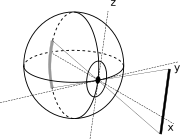
\includegraphics[scale=0.5]{3D-Eye-no-legend}
		\caption{Representação Esquemática do Olho Tridimensional. Ver referências dessa figura na Proposta de Iniciação Científica}
		\label{fig:Olho3D}
	\end{figure}
	
	\paragraph{}
	O algoritmo de renderização deve ser repetido \textbf{para cada ponto da tela}, sendo a ordem não importante, desde que a tela como um todo seja desenhada apenas depois que todos os pixels forem renderizados. Entretanto, por uma questão prática, escolhe-se desenhar a tela começando pelo pixel de índice $i=1$, e indo até o píxel de índice $i=n$.
	
	\paragraph{}
	\begin{table}
		\caption{Conjunto de variáveis necessárias para renderizar um único pixel na tela}\label{tab:var}
		\begin{tabular}{ll}
			\toprule[1.3pt]
			\thead{\textbf{Variável}} & \thead{\textbf{Descrição}} \\
			\midrule 
	    	\makecell{$p$} & \makecell{Ponto Visualizado.} \\
		    \makecell{$p_0$} & \makecell{Ponto do Foco de Captura. Por definição $p_0$ é a origem do sistema de coordenadas, \\
		    	porque assume-se que o foco de captura é o ponto central de representação.} \\
		    \makecell{$p_L$} & \makecell{Ponto da Fonte de Luz.} \\
		    \makecell{$p_i$-$p_f$} & \makecell{Segmento Visualizado.} \\
		    \makecell{$t_l$} & \makecell{Largura da tela (unidimensional).} \\
		    \makecell{$n$} & \makecell{Número de Pixels da Tela.} \\
		    \makecell{$\alpha$} & \makecell{Ângulo do Pixel renderizado.} \\
		    \makecell{$d$} & \makecell{Distância da tela ao Foco de Captura.} \\
		    \makecell{$d_c$} & \makecell{Distância do ponto visualizado ao foco de captura.} \\
		    \makecell{$d_L$} & \makecell{Distancia do ponto visualizado à fonte de luz.} \\
		    \makecell{$\phi$} & \makecell{Ângulo de incidência da luz na normal do Segmento Visualizado em $p$.} \\
		    \makecell{$(r_i, g_i, b_i)$} & \makecell{Vetor de cor original de $p$, valor intrínseco ao objeto representado \\ 
		    	pelo segmento visualizado.} \\
		    \makecell{$(r_f, g_f, b_f)$} & \makecell{Vetor de cor renderizado (final) de $p$.} \\
		    \makecell{$I_L(D)$} & \makecell{Taxa de iluminação, dependente da distância $D$ do ponto iluminado em relação \\
		    	à fonte de luz.} \\
		    \makecell{$I_d$} & \makecell{Taxa de iluminação difusa, constante para todos os pontos do ambiente.} \\
		    \makecell{$P_i$} & \makecell{Pixel, de índice $i$, a ser renderizado} \\
		    \makecell{$S$} & \makecell{Largura total da tela}\\
		    \makecell{$S_f$} & \makecell{Distância da borda da tela até a posição do foco de captura perante ela.} \\
		    \makecell{$i_i$} & \makecell{Índice do Pixel, apenas para diferenciar da unidade imaginária  ($i$).} \\
		    \bottomrule[1.3pt]
		\end{tabular}
	\end{table}

	Então, para cada pixel $i = 1, 2, ..., n$, deve-se implementar o seguinte algoritmo:
	
	\paragraph{1 - Identificação do ponto de renderização do pixel:}
	Cada pixel deve renderizar um ponto de acordo com o \textbf{Critério da Direção}: renderiza-se o ponto de algum segmento $p_i$-$p_f$ que intercepte a reta que passa pelo centro do pixel e pela origem (o ponto $p_0$, ou foco de captura) e que esteja mais próximo da origem. Todos os outros pontos que cumprirem a condição de estarem na reta determinada por $p_0$ e $P_i$ serão ignorados.
	
	Assim deve-se calcular:
	
	\begin{itemize}
		\item Reta de todos os pontos $r_\text{pixel} : r_\text{pixel} = (P_i - P_0) \cdot t$, $P_i = d \cdot \boldsymbol{e_x} + S_f \cdot \boldsymbol{e_y}$, $S_f = \frac{S}{2} - \frac{S}{n} \cdot i_i + \frac{S}{2n}$
		\item Retas de todos os segmentos renderizáveis: Para todo $p_i$, $p_f$ representado no espaço a ser renderizado. $p_i$ e $p_f$ representando segmentos renderizáveis, calcular as suas retas $r_\text{segmento}: r_\text{segmento} = (p_i + p_f \cdot t)$
		\item Pontos de interseção de $r_\text{pixel}$ e de $r_\text{segmento}$. Para calcular tal interseção, basta resolver os sistemas de equação de $r_\text{pixel}$ com cada $r_\text{segmento}$ e verificar se o valor no eixo $x$ de cada ponto encontrado está entre o valor de $x_{p_i}$ e $x_{p_f}$ correspondente a cada segmento cuja reta foi usada para se fazer tal interseção. 
		\item Distância de cada ponto de interseção encontrado em relação à origem.
	\end{itemize}
	 
	De todos os pontos identificados e com distância calculada, deve-se renderizar apenas aquele cuja distância em relação à origem for o menor. Esta é uma aplicação do \textbf{Critério da Distância}. Todos os outros pontos estão escondidos \textbf{atrás} deste.
	
	\paragraph{2 - Verificação se o ponto está iluminado ou em sombra:}
	Uma vez identificado o ponto, precisamos identificar o vetor que liga o Foco de Captura a esse ponto, e, também tal ponto à Fonte de Luz. Um vetor normal ao segmento,  $(p_i\text{-}p_f)^\bot$, passando pelo ponto $p$ identificado, também é necessário. Se os vetores $p_0$-$p$ e $p_{L}$-$p$ tiverem origem do mesmo lado do segmento $p_i$-$p_f$, então:
	
	$$\frac{\langle p_0\text{-}p , (p_i\text{-}p_f)^\bot \rangle}{\lvert \langle p_0\text{-}p , (p_i\text{-}p_f)^\bot \rangle \rvert} = \frac{\langle p_L\text{-}p , (p_i\text{-}p_f)^\bot \rangle}{\lvert \langle p_L\text{-}p , (p_i\text{-}p_f)^\bot \rangle \rvert}$$
	
	\paragraph{}
	Se os vetores $p_0\text{-}p$ e $p_L\text{-}p$ estiverem do mesmo lado, ou seja, se a igualdade acima valer, então o ponto é iluminado. Caso contrário, é ponto de sombra.
	
	\paragraph{}
	Entretanto, antes de se fazer essa verificação de sinal dos vetores e da normal, deve-se verificar se o ponto $p$ em questão é o primeiro a ser interceptado, a partir da Fonte de Luz, na reta $p_0$-$p_L$. Se esse não for o caso, como, por exemplo, os dos pontos $p_4$ e $p_5$, da Figura \ref{fig:rend}, o ponto é, automaticamente, um ponto de sombra, e nenhum cálculo adicional é necessário.
	
	\paragraph{3 - Cálculo da cor do pixel: }
	Se foi identificado se o pixel está representando um ponto iluminado ou um ponto de sombra, é necessário, então, definir qual cor o pixel irá assumir, e após essa definição, renderizar o pixel é apenas colori-lo integralmente com essa cor.
	
	\paragraph{}
	As duas primeiras variáveis a serem calculadas são:
	
	\paragraph{}
	A taxa de iluminação total do ponto renderizado: 

	\begin{equation} \label{eq:2}
		I_t =  \begin{cases} 
			min(I_d + I_L(D_L), 1), D_L = dist(p, F_L) = dist(p, p_L) & \text{se o ponto está iluminado} \\
			I_d & \text{se o ponto é de sombra} \\
		\end{cases} 
	\end{equation}

	Sendo $p_L$ o ponto da fonte de luz paralela $F_L$, que pode ser modelada como uma reta passando por $p_L$ (reta infinita, não apenas segmento), e $p_L$ pertencendo à reta $p$-$p_L$ perpendicular a $F_L$, lembrando que é $F_L$ que está fixa no espaço, não $p$-$p_L$, e, da equação \ref{eq:1}, assumindo $n = 2$ e $k = 2$:
	
	\begin{equation} \label{eq:3}
		I_L(D_L) = I(dist(p, p_L)) =  \frac{2}{(1+dist(p, p_L))^2}
	\end{equation}
	
	A distância $d(p, p_L)$ deve ter uma unidade de distância qualquer, mas, aqui, vamos considerar que existe uma unidade padrão e que as fórmulas todas apresentadas estão nessa unidade padrão.
	
	\paragraph{}
	E a intensidade de renderização na tela, que segue a mesma fórmula de intensidade da iluminação:
	
	\begin{equation} \label{eq:4}
		I_R \equiv I_D, I_R(D_0) = I(dist(p, p_0)) = \frac{2}{(1+dist(p, p_0))^2}
	\end{equation}
	
	\paragraph{}
	Uma vez que temos a Intensidade de Iluminação e a Intensidade de Renderização, podemos definir a cor final do pixel:
	
	\begin{equation}
		(r_f, g_f, b_f) = I_t \cdot I_R(D_0) \cdot (r_i, g_i, b_i), \text{para cada ponto $p$ na tela}.
	\end{equation}
	
	\paragraph{}
	Lembrando que $0 \le r_i < 256$, $0 \le g_i < 256$ e $0 \le b_i < 256$.
	
	\subsection{Iluminação Radial}
	
	\paragraph{} 
	Para a Fonte de Luz pontual, que permite uma iluminaçao radial, segue exatamente os mesmos princípios e cálculos de identificação dos pixels a serem renderizados, da sua intensidade luminosa e decaimento de intensidade de representação. 
	
	\begin{figure}[h]
		\centering
		\includegraphics[scale=0.8]{Renderizacao-2D-1D-radial}
		\caption{Identificando pontos de renderização.}
		\label{fig:rend-rad}
	\end{figure}
	
	\paragraph{}
	A única diferença é que $p_L$, ao invés de estar em uma reta infinita representando a fonte de luz, está em uma posição específica no espaço, e a distância $p$-$p_L$ é a distância do ponto $p$ ao próprio ponto $p_L$, já previamente definido, enquanto no caso da iluminação paralela, $p_L$ precisava ser tal que a reta $p$-$p_L$ fosse perpendicular à reta da fonte de luz.
	
	\paragraph{}
	Sendo assim, nenhuma informação adicional a respeito dos procedimentos para renderização nesse caso serão apresentados, pois seria pura redundância.
	
	\paragraph{}
	\begin{figure}[h]
		\centering
		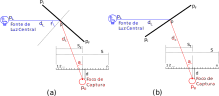
\includegraphics[scale=0.7]{radiosity-radial}
		\caption{Identificando pontos de renderização.}
		\label{fig:radio-rad}
	\end{figure}

	\section{Modelo Ampliado (1) - Ambiente Tridimensional em Tela Monodimensional}
	
	\paragraph{}
	A apresentação do Ambiente Bidimensional em Tela Monodimensional teve, como propósito, apenas lançar as bases para a representação de ambientes de dimensão mais alta em telas de dimensão inferiores, a uma diferença superior a um, como o caso desse modelo aqui apresentado.
	
	\begin{figure}
		\centering
		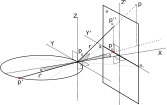
\includegraphics[scale=0.6]{Olho-Bidi-Detalhe}
		\caption{Captura de vetores de luz pelo olho bidimensional em ambiente tridimensional}
		\label{fig:olho-bidi}
	\end{figure}

	\paragraph{}
	No caso da representação de $\R^3$ em projeção em $\R$, a perda de informação é ainda mais severa do que a da projeção de $\R^2$ em $\R$ ou de $\R^3$ em $\R^2$. Além disso, pode haver sobreposição de representações, o que leva a algumas escolhas bastante severas a respeito de que informação iremos renunciar, para a imagem renderizada ainda fazer sentido. Através da \textbf{navegação}, entretanto, podemos definir mecanismos de recuperação da informação perdida.
	
	\paragraph{}
	Mas, faz sentido pensar em um ser bidimensional, com visão monodimensional, imerso em um espaço bidimensional? Podemos afirmar que sim, porque a visão dos animais é baseada na sensibilização de pontos (os cones e os bastonetes), organizados, dentro do olho, na forma de um reticulado. Se esse reticulado é bidimensional ou tridimensional, depende-se da conformação fisiológica do ser em particular.

	\paragraph{}
	O modelamento da renderização de um pixel em uma tela monodimensional em um ambiente tridimensional e, então, extender esse modelo para dimensões superiores, segue o que é apresentado na Figura \ref{fig:olho-bidi} abaixo, que representa o olho bidimensional imerso no ambiente tridimensional.
	
	\begin{figure}
		\centering
		
\includegraphics[scale=0.6]{refr-captura-luz}
		\caption{Exemplo de captura de luz de um ambiente tridimensional, para um bidimensional, em um material de altíssima refringência.}
		\label{fig:refr-cap}
	\end{figure}

	\paragraph{}
	A pergunta que não quer calar é se é possível para um ser bidimensional, imerso em um espaço tridimensional, enxergar figuras tridimensionais. Essa pergunta é bastante inadequada, porque em um ambiente tridimensional não é possível ter seres bidimensionais: o que é possível é ter seres achatados, cujos órgãos de visão são estruturados bidimensionalmente. É fisicamente factível a existência de uma retina bidimensional em um ser tridimensional achatado, conforme pode ser visto na Figura \ref{fig:refr-cap}, que apresenta o corte de um olho bidimensional, feito com material transparente de alta refringência, que pode captura todos os raios de luz que atingem o seu ponto de captura luminosa e os direciona para um objeto matemático com uma dimensão a menos.
	
	\paragraph{}
	Na Figura \ref{fig:refr-cap}, o ponto de entrada de luz é o representado pelo encontro dos eixos \textbf{X}, que aponta para a direita, \textbf{Y}, que aponta para dentro do papel, e \textbf{Z}, que, para respeitar a orientação da Regra da Mão Direita, aponta para cima. O raio de luz incide no corpo do olho com um ângulo de incidência $\phi$ e, como o olho é feito com material de alta refringência, uma parte da luz é refletida, e uma parte, com a intensidade igual à intensidade original multiplicada pelo cosseno do ângulo de incidência $\phi$ é capturado e retido dentro da estrutura do olho pelas propriedades da reflexão total.
	
	\paragraph{}
	Sabendo que há justificativa física para a construção de olhos que reduzem a dimensão do objeto de projeção - que no caso de um ambiente 3D seria uma linha, no caso de um ambiente 4D um plano, ou uma superfície bidimensional, e assim por diante - devemos, agora, avaliar como representar os pontos capturados por essa \textit{retina} unidimensional em um ambiente tridimensional.
	
	\paragraph{}
	Observando a Figura \ref{fig:olho-bidi}, vamos dar atenção ao ponto $p$, que é o ponto capturado. Para esse ponto ser capturado e impresso na tela, são utilizados os mesmos critérios apresentados para a Tela Unidimensional em um Ambiente Bidimensional:
	
	\paragraph{1 - Identificação do ponto de renderização do pixel:}
	Aqui, tanto quanto no caso do ambiente bidimensional, deve-se respeitar o \textbf{Critério da Direção}. Aqui temos a representação da tela como uma linha no espaço, entre $\alpha_0$-$\alpha_1$, conforme a Figura \ref{fig:olho-bidi}.
	
	\paragraph{2 - Verificação se o ponto está iluminado ou em sombra:}
	\paragraph{3 - Cálculo da cor do pixel: }
	
	\paragraph{}
	Entretanto, pode-se verificar, aqui, que cada pixel da tela irá renderizar todos pontos que possuem uma coordenada \textbf{Y} em comum - ou seja, para todos os pontos que se projetarem em $\alpha$ em uma determinada coordenada $(Y',Z')$, todos os pontos com o mesmo valor de \textbf{Y} vão ser renderizados no mesmo ponto. Para isso ser possível, todos esses pontos serão combinados utilizando-se a técnica de \textit{alpha-blending}. A combinação de todos esses pontos representa o que vai ser visualizado naquele ponto da tela (unidimensional no caso apresentado nessa seção).
	
	\section{Modelo Ampliado (2) - Ambiente Quadridimensional em Tela bidimensional}
	
	\paragraph{}
	\textbf{Continua...}
	
	\section{Modelo Ampliado (3) - Ambiente N-Dimensional em Tela M-dimensional}
	
	\paragraph{}
	\textbf{Continua...}
	
	\section{Múltiplas fontes de Luz e \textit{tinting}}
	
	\paragraph{}
	Essa seção apresenta a implementação da importante omissão do uso de múltiplas fontes de luz e do \textit{tinting}. O \textit{tinting} é a aplicação de fontes de luz coloridas, que alteram as cores dos objetos iluminados segundo regras específicas diferentes do \textit{alpha-blending} utilizado nas renderizações apresentadas acima. Já o uso de multiplas fontes de luz provoca um grande aumento de complexidade para a renderização de cada pixel da tela, ainda mais, considerando que cada fonte de luz pode ter uma cor diferente, alterando as regras de \textit{tinting}.
	
	\textbf{Continua...}
	
	\section{Conclusões e Próximos Passos}
	
	\paragraph{}
	\textbf{Continua...}

	
\end{document}
